% FRET ball vision: from camera images to the grasp pose.
%
% Build (from this folder):
%   python3 ../../../scripts/vision_algorithm_figures.py   # figures + data.tex
%   latexmk -pdf vision_algorithm.tex
%
% A Markdown version with the same content and numbers is generated as
% vision_algorithm.md from vision_algorithm.template.md.
\documentclass[11pt,a4paper]{article}

\usepackage[T1]{fontenc}
\usepackage[utf8]{inputenc}
\usepackage[english]{babel}
\usepackage{lmodern}
\usepackage{microtype}
\usepackage[margin=2.4cm]{geometry}
\usepackage{amsmath,amssymb,amsthm,mathtools,bm}
\usepackage{graphicx}
\usepackage{booktabs}
\usepackage{array}
\usepackage{float}
\usepackage[section]{placeins}
\usepackage[font=small,labelfont=bf]{caption}
\usepackage{subcaption}
\usepackage{xcolor}
\usepackage{tikz}
\usetikzlibrary{arrows.meta,positioning}
\usepackage[group-minimum-digits=5,group-digits=integer]{siunitx}
\usepackage[colorlinks=true,linkcolor=blue!50!black,citecolor=green!40!black,urlcolor=blue!60!black]{hyperref}

% Generated by scripts/vision_algorithm_figures.py -- do not edit.
\newcommand{\CircCircRf}{0.884}
\newcommand{\CircCircRba}{0.892}
\newcommand{\CircCircRda}{0.898}
\newcommand{\CircCircRga}{0.898}
\newcommand{\CircMecErrAboveHalfMax}{0.094}
\newcommand{\BiasOmxBiasMaxPx}{0.573}
\newcommand{\BiasOmxAlphaMaxDeg}{38.1}
\newcommand{\BiasOmxCheckMaxdiffPx}{0.000}
\newcommand{\BiasOmyBiasMaxPx}{1.390}
\newcommand{\BiasOmyAlphaMaxDeg}{40.2}
\newcommand{\BiasOmyCheckMaxdiffPx}{0.000}
\newcommand{\OmxCalOrth}{9.5e-11}
\newcommand{\OmxCalDet}{4.3e-11}
\newcommand{\OmxCalExt}{4.4e-11}
\newcommand{\OmxCalFx}{1.0e-08}
\newcommand{\OmxFx}{937.8321}
\newcommand{\OmxFovy}{42}
\newcommand{\OmxBallr}{20}
\newcommand{\OmxHsvBallFracInside}{100.00}
\newcommand{\OmxHsvBgFracInside}{0.00}
\newcommand{\OmxHsvBallHMedian}{34}
\newcommand{\OmxHsvBallSMedian}{196}
\newcommand{\OmxHsvBallVMedian}{231}
\newcommand{\OmxHsvBallHPab}{30}
\newcommand{\OmxHsvBallHPjj}{36}
\newcommand{\OmxHsvBallVPab}{130}
\newcommand{\OmxLU}{722.37}
\newcommand{\OmxLV}{327.41}
\newcommand{\OmxLUGt}{722.34}
\newcommand{\OmxLVGt}{327.45}
\newcommand{\OmxLRadiusPx}{20.88}
\newcommand{\OmxLAreaPx}{1305.0}
\newcommand{\OmxLPerimeterPx}{135.88}
\newcommand{\OmxLCirc}{0.8882}
\newcommand{\OmxLT}{0.9059}
\newcommand{\OmxLWeight}{0.4961}
\newcommand{\OmxLCentreErrPx}{0.05}
\newcommand{\OmxLIou}{0.984}
\newcommand{\OmxLDepth}{0.9059}
\newcommand{\OmxLTanIncidence}{0.889}
\newcommand{\OmxLNContours}{1}
\newcommand{\OmxLDcX}{0.08836}
\newcommand{\OmxLDwX}{0.37532}
\newcommand{\OmxLOX}{-0.120}
\newcommand{\OmxLPX}{220.01}
\newcommand{\OmxLDcY}{-0.03421}
\newcommand{\OmxLDwY}{-0.55199}
\newcommand{\OmxLOY}{0.300}
\newcommand{\OmxLPY}{-200.06}
\newcommand{\OmxLDcZ}{1.00000}
\newcommand{\OmxLDwZ}{-0.75062}
\newcommand{\OmxLOZ}{0.700}
\newcommand{\OmxLPZ}{20.00}
\newcommand{\OmxLEllA}{20.80}
\newcommand{\OmxLEllB}{20.71}
\newcommand{\OmxLEllBias}{0.043}
\newcommand{\OmxLEllAlpha}{5.41}
\newcommand{\OmxLEllDist}{0.9099}
\newcommand{\OmxLEllArea}{1353.5}
\newcommand{\OmxLSegpx}{1342}
\newcommand{\OmxLJAa}{-0.7199}
\newcommand{\OmxLJAb}{-0.8043}
\newcommand{\OmxLJBa}{-0.6441}
\newcommand{\OmxLJBb}{1.0072}
\newcommand{\OmxLJsig}{1.291}
\newcommand{\OmxRU}{764.56}
\newcommand{\OmxRV}{468.25}
\newcommand{\OmxRUGt}{764.63}
\newcommand{\OmxRVGt}{468.04}
\newcommand{\OmxRRadiusPx}{25.21}
\newcommand{\OmxRAreaPx}{1898.5}
\newcommand{\OmxRPerimeterPx}{162.61}
\newcommand{\OmxRCirc}{0.9022}
\newcommand{\OmxRT}{0.7550}
\newcommand{\OmxRWeight}{0.5039}
\newcommand{\OmxRCentreErrPx}{0.22}
\newcommand{\OmxRIou}{0.988}
\newcommand{\OmxRDepth}{0.7551}
\newcommand{\OmxRTanIncidence}{0.521}
\newcommand{\OmxRNContours}{1}
\newcommand{\OmxRDcX}{0.13335}
\newcommand{\OmxRDwX}{0.45006}
\newcommand{\OmxROX}{-0.120}
\newcommand{\OmxRPX}{219.80}
\newcommand{\OmxRDcY}{0.11596}
\newcommand{\OmxRDwY}{0.13238}
\newcommand{\OmxROY}{-0.300}
\newcommand{\OmxRPY}{-200.05}
\newcommand{\OmxRDcZ}{1.00000}
\newcommand{\OmxRDwZ}{-0.90064}
\newcommand{\OmxROZ}{0.700}
\newcommand{\OmxRPZ}{20.00}
\newcommand{\OmxREllA}{25.23}
\newcommand{\OmxREllB}{24.85}
\newcommand{\OmxREllBias}{0.116}
\newcommand{\OmxREllAlpha}{10.02}
\newcommand{\OmxREllDist}{0.7668}
\newcommand{\OmxREllArea}{1969.7}
\newcommand{\OmxRSegpx}{1946}
\newcommand{\OmxRJAa}{0.4374}
\newcommand{\OmxRJAb}{-0.7859}
\newcommand{\OmxRJBa}{-0.6759}
\newcommand{\OmxRJBb}{-0.4309}
\newcommand{\OmxRJsig}{0.905}
\newcommand{\OmxGtX}{220.00}
\newcommand{\OmxFuX}{219.91}
\newcommand{\OmxGtY}{-200.00}
\newcommand{\OmxFuY}{-200.05}
\newcommand{\OmxGtZ}{20.00}
\newcommand{\OmxFuZ}{20.00}
\newcommand{\OmxExXyerr}{0.108}
\newcommand{\OmxExZerr}{0.000}
\newcommand{\OmxJacFd}{3.8e-13}
\newcommand{\OmxMcEmpMinMm}{0.329}
\newcommand{\OmxMcEmpMaxMm}{0.382}
\newcommand{\OmxMcPredMinMm}{0.327}
\newcommand{\OmxMcPredMaxMm}{0.380}
\newcommand{\OmxMcFrobRel}{0.010}
\newcommand{\OmxDzShift}{0.578}
\newcommand{\OmxIkHoverMm}{0.004}
\newcommand{\OmxIkGraspMm}{0.000}
\newcommand{\OmxIkLiftMm}{0.003}
\newcommand{\OccVisibleFrac}{12.1}
\newcommand{\OccCentreErrPx}{16.28}
\newcommand{\OccCirc}{0.51}
\newcommand{\OccRadiusPx}{13.73}
\newcommand{\OccAPx}{22.38}
\newcommand{\occMonoErr}{0.14}
\newcommand{\occLeftErr}{17.61}
\newcommand{\occLeftW}{0.363}
\newcommand{\occFusedErr}{6.40}
\newcommand{\OmxMecGap}{1.0e-04}
\newcommand{\OmxSwN}{9}
\newcommand{\OmxSwDet}{9}
\newcommand{\OmxSwMedian}{0.14}
\newcommand{\OmxSwMax}{6.40}
\newcommand{\OmxGridN}{208}
\newcommand{\OmxGridDet}{208}
\newcommand{\OmxGridDual}{165}
\newcommand{\OmxGridMedian}{0.25}
\newcommand{\OmxGridPjf}{7.49}
\newcommand{\OmxGridMax}{17.20}
\newcommand{\OmxGridClearN}{93}
\newcommand{\OmxGridClearMax}{0.73}
\newcommand{\OmxGridClearMedian}{0.14}
\newcommand{\OmyCalOrth}{1.3e-10}
\newcommand{\OmyCalDet}{7.6e-11}
\newcommand{\OmyCalExt}{4.9e-11}
\newcommand{\OmyCalFx}{4.6e-08}
\newcommand{\OmyFx}{869.1169}
\newcommand{\OmyFovy}{45}
\newcommand{\OmyBallr}{43}
\newcommand{\OmyHsvBallFracInside}{99.98}
\newcommand{\OmyHsvBgFracInside}{0.01}
\newcommand{\OmyHsvBallHMedian}{34}
\newcommand{\OmyHsvBallSMedian}{196}
\newcommand{\OmyHsvBallVMedian}{230}
\newcommand{\OmyHsvBallHPab}{30}
\newcommand{\OmyHsvBallHPjj}{36}
\newcommand{\OmyHsvBallVPab}{125}
\newcommand{\OmyLU}{752.67}
\newcommand{\OmyLV}{326.21}
\newcommand{\OmyLUGt}{752.58}
\newcommand{\OmyLVGt}{326.46}
\newcommand{\OmyLRadiusPx}{29.46}
\newcommand{\OmyLAreaPx}{2609.0}
\newcommand{\OmyLPerimeterPx}{191.34}
\newcommand{\OmyLCirc}{0.8955}
\newcommand{\OmyLT}{1.2837}
\newcommand{\OmyLWeight}{0.5015}
\newcommand{\OmyLCentreErrPx}{0.27}
\newcommand{\OmyLIou}{0.991}
\newcommand{\OmyLDepth}{1.2834}
\newcommand{\OmyLTanIncidence}{0.955}
\newcommand{\OmyLNContours}{1}
\newcommand{\OmyLDcX}{0.13021}
\newcommand{\OmyLDwX}{0.41307}
\newcommand{\OmyLOX}{-0.180}
\newcommand{\OmyLPX}{350.26}
\newcommand{\OmyLDcY}{-0.03831}
\newcommand{\OmyLDwY}{-0.56126}
\newcommand{\OmyLOY}{0.420}
\newcommand{\OmyLPY}{-300.48}
\newcommand{\OmyLDcZ}{1.00000}
\newcommand{\OmyLDwZ}{-0.72992}
\newcommand{\OmyLOZ}{0.980}
\newcommand{\OmyLPZ}{43.00}
\newcommand{\OmyLEllA}{29.40}
\newcommand{\OmyLEllB}{29.14}
\newcommand{\OmyLEllBias}{0.132}
\newcommand{\OmyLEllAlpha}{7.72}
\newcommand{\OmyLEllDist}{1.2951}
\newcommand{\OmyLEllArea}{2691.5}
\newcommand{\OmyLSegpx}{2668}
\newcommand{\OmyLJAa}{-1.0050}
\newcommand{\OmyLJAb}{-1.3653}
\newcommand{\OmyLJBa}{-1.0823}
\newcommand{\OmyLJBb}{1.5035}
\newcommand{\OmyLJsig}{2.039}
\newcommand{\OmyRU}{769.25}
\newcommand{\OmyRV}{470.18}
\newcommand{\OmyRUGt}{769.31}
\newcommand{\OmyRVGt}{469.67}
\newcommand{\OmyRRadiusPx}{35.82}
\newcommand{\OmyRAreaPx}{3851.0}
\newcommand{\OmyRPerimeterPx}{233.14}
\newcommand{\OmyRCirc}{0.8903}
\newcommand{\OmyRT}{1.0625}
\newcommand{\OmyRWeight}{0.4985}
\newcommand{\OmyRCentreErrPx}{0.52}
\newcommand{\OmyRIou}{0.991}
\newcommand{\OmyRDepth}{1.0630}
\newcommand{\OmyRTanIncidence}{0.579}
\newcommand{\OmyRNContours}{1}
\newcommand{\OmyRDcX}{0.14929}
\newcommand{\OmyRDwX}{0.49815}
\newcommand{\OmyROX}{-0.180}
\newcommand{\OmyRPX}{349.31}
\newcommand{\OmyRDcY}{0.12735}
\newcommand{\OmyRDwY}{0.11272}
\newcommand{\OmyROY}{-0.420}
\newcommand{\OmyRPY}{-300.23}
\newcommand{\OmyRDcZ}{1.00000}
\newcommand{\OmyRDwZ}{-0.88184}
\newcommand{\OmyROZ}{0.980}
\newcommand{\OmyRPZ}{43.00}
\newcommand{\OmyREllA}{35.86}
\newcommand{\OmyREllB}{35.19}
\newcommand{\OmyREllBias}{0.279}
\newcommand{\OmyREllAlpha}{11.08}
\newcommand{\OmyREllDist}{1.0832}
\newcommand{\OmyREllArea}{3963.7}
\newcommand{\OmyRSegpx}{3919}
\newcommand{\OmyRJAa}{0.6066}
\newcommand{\OmyRJAb}{-1.2644}
\newcommand{\OmyRJBa}{-1.0615}
\newcommand{\OmyRJBb}{-0.5816}
\newcommand{\OmyRJsig}{1.408}
\newcommand{\OmyGtX}{350.00}
\newcommand{\OmyFuX}{349.79}
\newcommand{\OmyGtY}{-300.00}
\newcommand{\OmyFuY}{-300.36}
\newcommand{\OmyGtZ}{43.00}
\newcommand{\OmyFuZ}{43.00}
\newcommand{\OmyExXyerr}{0.418}
\newcommand{\OmyExZerr}{0.000}
\newcommand{\OmyJacFd}{7.1e-13}
\newcommand{\OmyMcEmpMinMm}{0.502}
\newcommand{\OmyMcEmpMaxMm}{0.603}
\newcommand{\OmyMcPredMinMm}{0.500}
\newcommand{\OmyMcPredMaxMm}{0.600}
\newcommand{\OmyMcFrobRel}{0.011}
\newcommand{\OmyDzShift}{0.651}
\newcommand{\OmyIkHoverMm}{0.000}
\newcommand{\OmyIkGraspMm}{0.001}
\newcommand{\OmyIkLiftMm}{0.000}
\newcommand{\OmyMecGap}{1.0e-04}
\newcommand{\OmySwN}{9}
\newcommand{\OmySwDet}{8}
\newcommand{\OmySwMedian}{0.50}
\newcommand{\OmySwMax}{3.69}
\newcommand{\OmyGridN}{210}
\newcommand{\OmyGridDet}{199}
\newcommand{\OmyGridDual}{100}
\newcommand{\OmyGridMedian}{0.75}
\newcommand{\OmyGridPjf}{30.37}
\newcommand{\OmyGridMax}{37.97}
\newcommand{\OmyGridClearN}{38}
\newcommand{\OmyGridClearMax}{0.70}
\newcommand{\OmyGridClearMedian}{0.43}

\makeatletter
\newcommand{\generatedrows}[1]{\@@input #1 }
\makeatother

\setlength{\emergencystretch}{3em}

\newtheorem{proposition}{Proposition}
\newtheorem{corollary}[proposition]{Corollary}
\theoremstyle{definition}
\newtheorem{definition}{Definition}
\theoremstyle{remark}
\newtheorem{remark}{Remark}

\newcommand{\R}{\mathbb{R}}
\newcommand{\Z}{\mathbb{Z}}
\newcommand{\T}{^{\mkern-1.5mu\mathsf{T}}}
\newcommand{\vect}[1]{\bm{#1}}
\newcommand{\ez}{\vect{e}_z}
\newcommand{\code}[1]{\texttt{\detokenize{#1}}}
\DeclareMathOperator{\HSV}{hsv}
\DeclareMathOperator{\MEC}{MEC}
\DeclareMathOperator*{\argmax}{arg\,max}
\DeclareMathOperator*{\argmin}{arg\,min}

\title{\textbf{Computer vision for pick-and-place in FRET}\\[2pt]
\large From camera images to the ball grasp pose:\\
mathematical model, implementation, and error analysis}
\author{FRET --- \texttt{fret.vision} module}
\date{October 2026}

\begin{document}
\maketitle

\begin{abstract}
\noindent
This document gives a mathematically rigorous description of the vision
algorithm FRET uses to locate a ball on the table and turn that location into
grasp targets for the OpenMANIPULATOR-X (OM-X) and OpenMANIPULATOR-Y (OMY)
arms. The full chain is: rendering two calibrated MuJoCo cameras;
thresholding in HSV space; morphological filtering; contour extraction and
selection by circularity; centre estimation with the minimum enclosing circle;
back-projection of the pixel as a world ray; intersection with the horizontal
plane that contains the ball centre; weighted fusion of the views; and
inverse kinematics of the fingertip midpoint. For each stage we give the
formulation, the assumptions, and propositions with proofs (shape of the
projected sphere silhouette, perspective bias, behaviour of the minimum
enclosing circle under occlusion, digital limit of circularity, Jacobian of
the plane lift). Every number was produced by running the repository code
(\code{scripts/vision_algorithm_figures.py}), and every closed form was checked
numerically against the implementation.
\end{abstract}

\tableofcontents
\newpage

%=====================================================================
\section{Overview}
\label{sec:overview}
%=====================================================================

The \code{fret.vision} module solves the following problem. Given RGB images
from $N\geq1$ calibrated cameras, estimate the world-frame position
$\vect p^\star\in\R^3$ of the centre of a ball of known radius $r$ resting on a
horizontal table of known height $z_{\text{table}}$. The controller then uses
the estimate $\hat{\vect p}$ to compute the approach, grasp, and lift joint
configurations.

Figure~\ref{fig:pipeline} summarises the flow. The code is split into three
stages behind algorithm-agnostic protocols (\code{fret/vision/protocols.py}):
a \emph{detector} (image $\to$ pixel hypotheses), an optional \emph{tracker}
(unused in the current configuration), and a \emph{pose lifter} (pixels $\to$
world). Orchestration lives in \code{BallVisionPipeline.process}
(\code{fret/vision/pipeline.py}); the concrete wiring is in
\code{fret/vision/factory.py}.

\begin{figure}[ht]
\centering
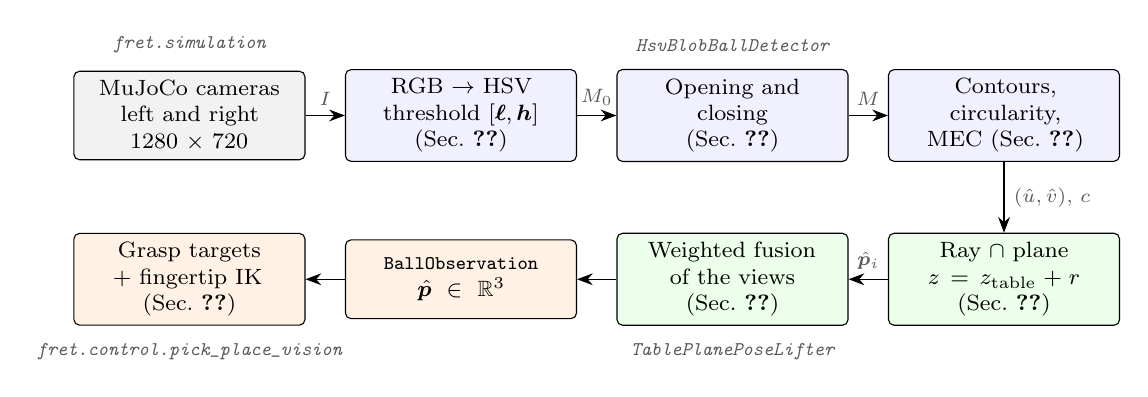
\begin{tikzpicture}[
  node distance=4mm and 5mm,
  blk/.style={draw, rounded corners=2pt, fill=#1, align=center,
              font=\footnotesize, minimum height=10mm, text width=27mm},
  blk/.default={blue!6},
  lab/.style={font=\scriptsize\itshape, text=black!65},
  >={Stealth[length=2mm]}
]
\node[blk=gray!10] (cam) {MuJoCo cameras\\ left and right\\ $1280\times720$};
\node[blk, right=of cam] (hsv) {RGB $\to$ HSV\\ threshold $[\vect\ell,\vect h]$\\ (Sec.~\ref{sec:segmentation})};
\node[blk, right=of hsv] (morph) {Opening and\\ closing\\ (Sec.~\ref{sec:morphology})};
\node[blk, right=of morph] (cont) {Contours,\\ circularity,\\ MEC (Sec.~\ref{sec:contours})};
\node[blk=green!8, below=9mm of cont] (lift) {Ray $\cap$ plane\\ $z=z_{\text{table}}+r$\\ (Sec.~\ref{sec:lift})};
\node[blk=green!8, left=of lift] (fuse) {Weighted fusion\\ of the views\\ (Sec.~\ref{sec:fusion})};
\node[blk=orange!10, left=of fuse] (obs) {{\scriptsize\code{BallObservation}}\\ $\hat{\vect p}\in\R^3$};
\node[blk=orange!10, left=of obs] (ik) {Grasp targets\\ + fingertip IK\\ (Sec.~\ref{sec:grasp})};
\draw[->] (cam) -- node[lab, above]{$I$} (hsv);
\draw[->] (hsv) -- node[lab, above]{$M_0$} (morph);
\draw[->] (morph) -- node[lab, above]{$M$} (cont);
\draw[->] (cont) -- node[lab, right]{$(\hat u,\hat v),\,c$} (lift);
\draw[->] (lift) -- node[lab, above]{$\hat{\vect p}_i$} (fuse);
\draw[->] (fuse) -- (obs);
\draw[->] (obs) -- (ik);
\node[lab, above=1mm of cam] {\code{fret.simulation}};
\node[lab, above=1mm of morph] {\code{HsvBlobBallDetector}};
\node[lab, below=1mm of fuse] {\code{TablePlanePoseLifter}};
\node[lab, below=1mm of ik] {\code{fret.control.pick_place_vision}};
\end{tikzpicture}
\caption{End-to-end flow from images to grasp. Blue: image-space detector;
green: world geometry; orange: control consumers. Each view is processed
independently until fusion.}
\label{fig:pipeline}
\end{figure}

\paragraph{Scene.} In the pick-and-place cells (OM-X and OMY), two cameras
are mounted on the top corners of a structural gate behind the arm
(\code{docs/vision/camera-layout.md}). The ball is yellow-green (material
colour $\text{RGBA}=(0.85, 0.92, 0.20, 1)$) with radius \SI{\OmxBallr}{mm} in
the OM-X cell and \SI{\OmyBallr}{mm} in the OMY cell. Figure~\ref{fig:cameras}
shows both views at the OM-X default pick pose, and Figure~\ref{fig:overview}
shows the final estimate overlaid on the scene.

\begin{figure}[ht]
\centering
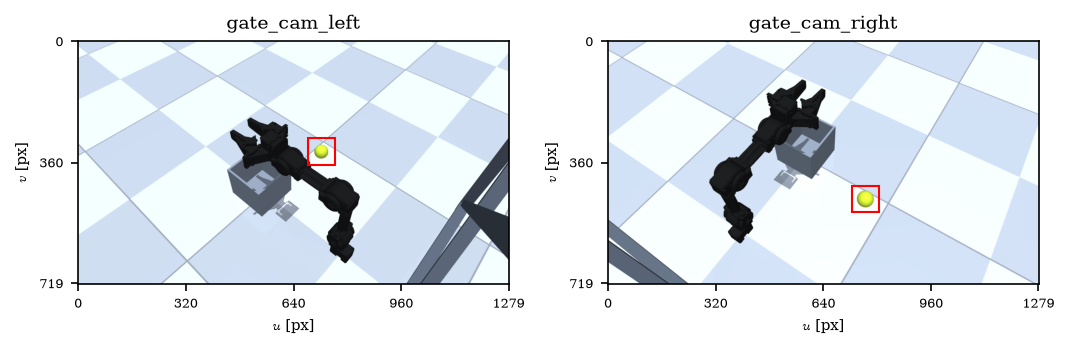
\includegraphics[width=\linewidth]{figures/cameras_omx.png}
\caption{Images rendered by the two gate cameras (OM-X, ball at
$(0.22, -0.20)$\,m). The red square marks the region enlarged in
Figure~\ref{fig:mask}.}
\label{fig:cameras}
\end{figure}

\begin{figure}[ht]
\centering
\begin{subfigure}{0.49\linewidth}
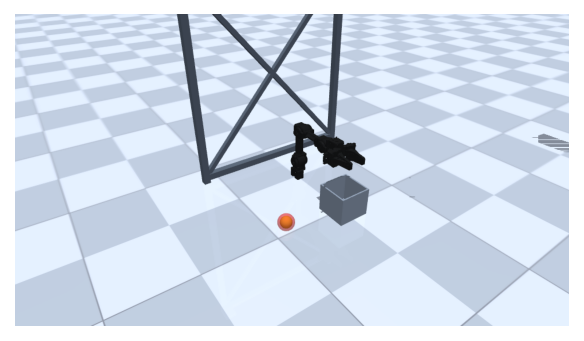
\includegraphics[width=\linewidth]{figures/overview_omx.png}
\caption{OM-X}
\end{subfigure}\hfill
\begin{subfigure}{0.49\linewidth}
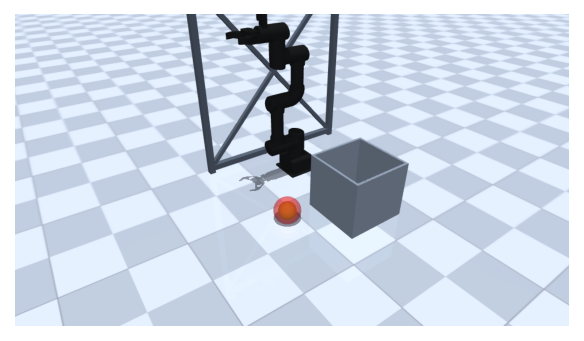
\includegraphics[width=\linewidth]{figures/overview_omy.png}
\caption{OMY}
\end{subfigure}
\caption{Cell overview. The translucent red sphere (\code{cv_ball_ghost},
visual only) is placed at the vision estimate $\hat{\vect p}$; the real yellow
ball sits inside it.}
\label{fig:overview}
\end{figure}

\paragraph{Notation.} Vectors are bold; $\ez=(0,0,1)\T$;
$\tilde{\vect u}=(u,v,1)\T$ are homogeneous pixel coordinates;
$[\,\cdot\,]_{xy}$ keeps the first two components. Angles are in radians
unless stated. Subscripts $L$ and $R$ refer to the left
(\code{gate_cam_left}) and right (\code{gate_cam_right}) cameras.

%=====================================================================
\section{Camera model}
\label{sec:camera}
%=====================================================================

\subsection{Frames}

Three frames are used: the world $\{W\}$ (origin at the arm base, $x$
forward, $z$ up); the MuJoCo camera $\{M\}$, which looks along $-z_M$ with
$y_M$ up in the image; and the OpenCV optical camera $\{C\}$, with $x_C$ to the
right, $y_C$ down, and $z_C$ into the scene. The whole pipeline works in
$\{C\}$.

MuJoCo provides the optical centre $\vect O\in\R^3$ (\code{cam_xpos}) and the
matrix $R_M\in SO(3)$ (\code{cam_xmat}), whose columns are the axes of $\{M\}$
expressed in $\{W\}$. Since $x_C=x_M$, $y_C=-y_M$, and $z_C=-z_M$,
\begin{equation}
R \;=\; R_M\,\operatorname{diag}(1,-1,-1),
\qquad
T_{WC} = \begin{bmatrix} R & \vect O\\ \vect 0\T & 1\end{bmatrix},
\label{eq:mj2cv}
\end{equation}
implemented in \code{mujoco_xmat_to_opencv_rotation}
(\code{fret/simulation/mujoco_camera.py}). $R$ is still a rotation: it is a
product of orthogonal matrices and $\det R=\det R_M\cdot(1)(-1)(-1)=1$. The
transform maps camera coordinates to world coordinates:
$\vect x_W=R\,\vect x_C+\vect O$.

\subsection{Pinhole projection and intrinsics}

With the intrinsic matrix
\begin{equation}
K=\begin{bmatrix} f_x & 0 & c_x\\ 0 & f_y & c_y\\ 0&0&1\end{bmatrix},
\end{equation}
a point $\vect x_W$ in front of the camera projects to
\begin{equation}
\vect x_C = R\T(\vect x_W-\vect O)=(X,Y,Z)\T,\qquad
u = f_x\frac{X}{Z}+c_x,\quad v=f_y\frac{Y}{Z}+c_y,\quad Z>0.
\label{eq:proj}
\end{equation}
The simulator has no lens distortion, and \code{CameraIntrinsics}
deliberately omits distortion coefficients.

MuJoCo defines a camera by its vertical field of view $\phi_y$
(\code{fovy}). On the plane $Z=1$ the visible half-height is
$\tan(\phi_y/2)$, which spans $H/2$ pixels; with square pixels,
\begin{equation}
f_x=f_y=f=\frac{H/2}{\tan(\phi_y/2)},\qquad
c_x=\frac{W-1}{2},\quad c_y=\frac{H-1}{2}
\label{eq:fovy}
\end{equation}
(\code{intrinsics_from_fovy}). The principal point uses the convention that
pixel $(i,j)$ is centred at integer coordinates $(i,j)$, the same convention
OpenCV uses for contours. For $H=720$: with $\phi_y=\ang{\OmxFovy}$ (OM-X),
$f=360/\tan(\ang{21})=\num{\OmxFx}$\,px; with $\phi_y=\ang{\OmyFovy}$ (OMY),
$f=360/\tan(\ang{22.5})=\num{\OmyFx}$\,px. In both cases
$(c_x,c_y)=(\num{639.5},\num{359.5})$.

\paragraph{Calibration consistency.} The $K$ and $T_{WC}$ of each camera are
stored in the YAML configuration of each cell (Appendix~\ref{app:params}).
Against the loaded MuJoCo model, the largest difference between the YAML
$T_{WC}$ and the one computed from the model is \num{\OmxCalExt} (OM-X) and
\num{\OmyCalExt} (OMY); the difference in $f$ and $c$ is
$\leq\num{\OmyCalFx}$\,px; and $\max|R\T R-I|\leq\num{\OmyCalOrth}$ with
$|\det R-1|\leq\num{\OmyCalDet}$. The calibration used by the pipeline
therefore matches the rendered geometry up to YAML rounding.

%=====================================================================
\section{Colour segmentation in HSV space}
\label{sec:segmentation}
%=====================================================================

\subsection{RGB to HSV conversion (OpenCV, 8 bits)}

Let $I:\Omega\to\{0,\dots,255\}^3$ be the RGB image, with
$\Omega=\{0,\dots,W-1\}\times\{0,\dots,H-1\}$. For a pixel $(R,G,B)$ let
$M_{\max}=\max(R,G,B)$, $m=\min(R,G,B)$, and $\Delta=M_{\max}-m$. OpenCV computes
\begin{align}
V &= M_{\max},\qquad
S = \begin{cases} 255\,\Delta/M_{\max}, & M_{\max}>0\\ 0,& M_{\max}=0\end{cases}\\
H' &= \begin{cases}
60\,(G-B)/\Delta, & M_{\max}=R\\
120+60\,(B-R)/\Delta, & M_{\max}=G\\
240+60\,(R-G)/\Delta, & M_{\max}=B
\end{cases}\quad (H'\leftarrow H'+360 \text{ if } H'<0),
\qquad H = H'/2,
\end{align}
rounded to integers. $H\in\{0,\dots,179\}$ is the hue in degrees divided by
two, and $S,V\in\{0,\dots,255\}$. The code converts RGB$\to$BGR$\to$HSV
(\code{_to_bgr} and \code{cv2.cvtColor}).

\paragraph{Example.} The ball's diffuse colour, $(217,235,51)$, has
$M_{\max}=G=235$, $m=51$, and $\Delta=184$. Hence $V=235$,
$S=255\cdot184/235\approx199.7\to200$, and
$H'=120+60(51-217)/184\approx65.9$, so $H=33$. \code{cv2.cvtColor} returns
exactly $(33,200,235)$.

\subsection{Threshold}

\begin{definition}[Colour mask]
Given bounds $\vect\ell,\vect h\in\{0,\dots,255\}^3$, the initial mask is
\begin{equation}
M_0(\vect x) = \begin{cases}255, & \vect\ell\preceq \HSV(I(\vect x))\preceq\vect h\\ 0,&\text{otherwise,}\end{cases}
\end{equation}
where $\preceq$ is the component-wise order with inclusive bounds
(\code{cv2.inRange}). If the configuration defines a second range
$[\vect\ell',\vect h']$, then $M_0\leftarrow M_0\vee M_0'$. The second range exists
because hue is circular: a red object occupies both $H\approx0$ and
$H\approx179$ and needs two intervals.
\end{definition}

In the gate cells, $\vect\ell=(20,40,40)$ and $\vect h=(50,255,255)$, with no
second range. Figure~\ref{fig:hsv} justifies the choice with data. The ball
pixels, identified by MuJoCo's segmentation render (the ground truth), lie in
$H\in[\num{\OmxHsvBallHPab},\num{\OmxHsvBallHPjj}]$ (1st and 99th
percentiles), with median $(H,S,V)=(\num{\OmxHsvBallHMedian},
\num{\OmxHsvBallSMedian},\num{\OmxHsvBallVMedian})$. The floor and the gate sit
at $H\approx90$--$120$ or have low $S$. At the default pose,
\SI{\OmxHsvBallFracInside}{\percent} of ball pixels fall inside the threshold
box, and \SI{\OmxHsvBgFracInside}{\percent} of an \num{80000}-pixel background
sample does (OMY: \SI{\OmyHsvBallFracInside}{\percent} and
\SI{\OmyHsvBgFracInside}{\percent}). The ball's minimum $V$
(\num{\OmxHsvBallVPab}, on the shaded side) is well above $\ell_V=40$, which
leaves room for lighting variation.

\begin{figure}[ht]
\centering
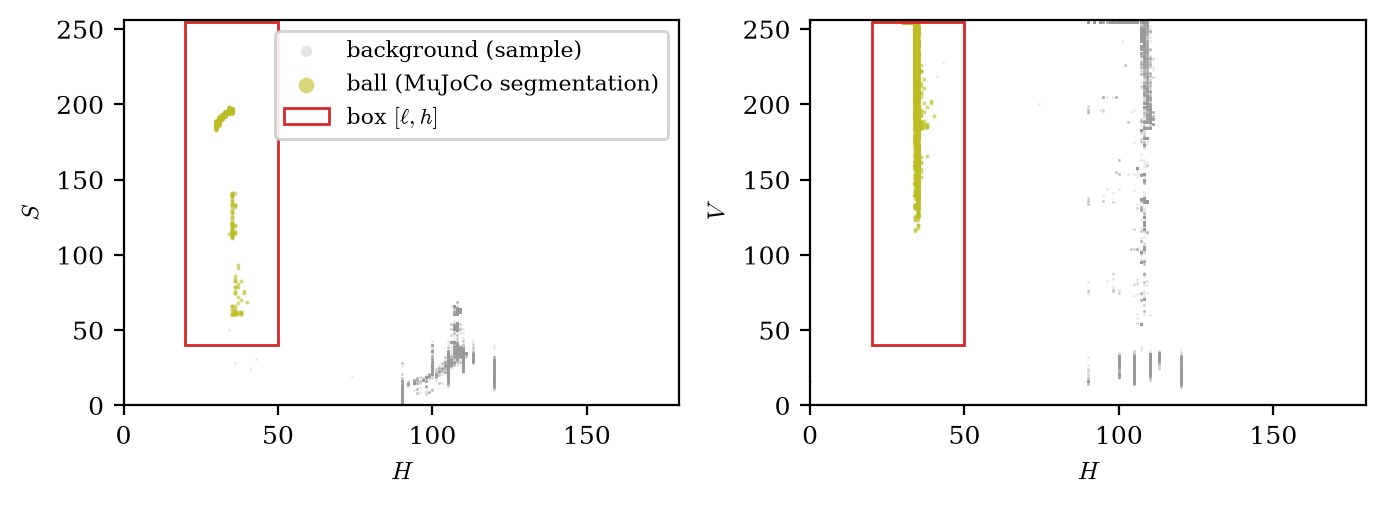
\includegraphics[width=0.92\linewidth]{figures/hsv_omx.png}
\caption{Ball pixels (olive, MuJoCo segmentation labels) and a background
sample (grey) in the $H$--$S$ and $H$--$V$ planes, with the OM-X threshold box
$[\vect\ell,\vect h]$. Both cameras are included.}
\label{fig:hsv}
\end{figure}

%=====================================================================
\section{Morphological filtering}
\label{sec:morphology}
%=====================================================================

Identify the binary mask with the set $X=\{\vect x\in\Omega:M_0(\vect
x)\neq0\}\subset\Z^2$. Let $B\subset\Z^2$ be a symmetric structuring element
($B=-B$) centred at the origin, and $B_{\vect x}=\vect x+B$.

\begin{definition}
Erosion $X\ominus B=\{\vect x: B_{\vect x}\subseteq X\}$; dilation
$X\oplus B=\{\vect x: B_{\vect x}\cap X\neq\emptyset\}$; opening
$X\circ B=(X\ominus B)\oplus B$; closing $X\bullet B=(X\oplus B)\ominus B$.
\end{definition}

The detector computes $M=(M_0\circ B)\bullet B$ (\code{mask_for_frame}), with
the structuring element returned by
\[
\text{\code{cv2.getStructuringElement(cv2.MORPH_ELLIPSE, (5, 5))}}\,:\qquad
B=\begin{bmatrix}
0&0&1&0&0\\1&1&1&1&1\\1&1&1&1&1\\1&1&1&1&1\\0&0&1&0&0
\end{bmatrix}.
\]

\begin{proposition}[Properties used]
\label{prop:morph}
(i) $X\circ B=\bigcup\{B_{\vect y}: B_{\vect y}\subseteq X\}\subseteq X$: opening
keeps exactly the points covered by some translate of $B$ that fits inside
$X$. (ii) $X\subseteq X\bullet B$ and $(X\bullet B)^c=X^c\circ B$. (iii) Both
operations are increasing and idempotent.
\end{proposition}
\begin{proof}
(i) $\vect z\in(X\ominus B)\oplus B$ if and only if there is $\vect y$ with
$B_{\vect y}\subseteq X$ and $\vect z\in B_{\vect y}$ (by symmetry of $B$).
(ii) By the duality $(X\oplus B)^c=X^c\ominus B$,
$(X\bullet B)^c=(X^c\ominus B)\oplus B=X^c\circ B$; the inclusion follows from
(i) applied to $X^c$. (iii) This is the classical result of Matheron and
Serra \cite{serra1982}.
\end{proof}

In practice, by Proposition~\ref{prop:morph}(i), opening deletes any
false-positive component that cannot contain a copy of $B$ (isolated pixels,
1--2\,px-wide lines on object edges). By (ii), closing fills holes and notches
in the complement that cannot contain $B$, such as a specular highlight or the
cut left by a thin edge in front of the ball. For an unoccluded ball of radius
$\approx20$--$36$\,px, both operations barely change the silhouette
(Figure~\ref{fig:mask}).

\begin{figure}[ht]
\centering
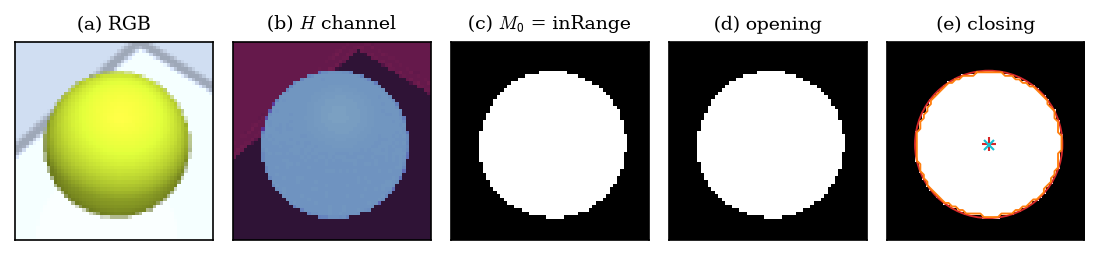
\includegraphics[width=\linewidth]{figures/mask_stages_omx.png}
\caption{Detector stages on the left camera (OM-X, default pose),
$56\times56$\,px crop. (e) External contour (orange), minimum enclosing circle
(red), and estimated centre ($+$). The cyan $\times$ is the exact projection of
the ball centre by Eq.~\eqref{eq:proj}.}
\label{fig:mask}
\end{figure}

%=====================================================================
\section{Contours, circularity, and centre}
\label{sec:contours}
%=====================================================================

\subsection{Contour extraction}

The detector extracts the outer borders of the 8-connected components of $M$
with the Suzuki--Abe border-following algorithm \cite{suzuki1985}
(\code{cv2.findContours}, mode \code{RETR_EXTERNAL}). Each contour is a closed
polygon $\mathcal P=(\vect q_0,\dots,\vect q_{n-1})$ whose vertices are border
pixel centres. \code{CHAIN_APPROX_SIMPLE} only removes intermediate vertices
of horizontal, vertical, or diagonal runs, so the polygon (as a subset of the
plane) is unchanged.

\subsection{Area, perimeter, and circularity}

\begin{equation}
A(\mathcal P)=\frac12\left|\sum_{k=0}^{n-1}\left(x_k y_{k+1}-x_{k+1}y_k\right)\right|,\qquad
P(\mathcal P)=\sum_{k=0}^{n-1}\|\vect q_{k+1}-\vect q_k\|,\qquad
c=\frac{4\pi A}{P^2},
\label{eq:circ}
\end{equation}
with indices modulo $n$ (\code{contourArea}, \code{arcLength},
\code{_circularity}). Because the vertices lie on the lattice $\Z^2$, Pick's
theorem gives, for a simple polygon, $A=I+B_\partial/2-1$, with $I$ interior
lattice points and $B_\partial$ lattice points on the border. So $A$ is about
half a pixel layer below the pixel count of the component. In the example of
Section~\ref{sec:example}, $A=\num{\OmxLAreaPx}$ against \num{\OmxLSegpx}
visible ball pixels in the reference segmentation and \num{\OmxLEllArea}\,px$^2$
of theoretical silhouette area.

By the isoperimetric inequality, $P^2\geq4\pi A$ for any closed plane curve,
with equality only for the circle. Hence $c\in(0,1]$, and $c=1$ characterises
the disk in the continuum. In the digital case the attainable maximum is
lower:

\begin{proposition}[Digital limit of circularity]
\label{prop:circ-digital}
Let $\mathcal P_R$ be the outer contour of a digitised disk of radius $R$. As
$R\to\infty$,
\begin{equation}
\frac{P(\mathcal P_R)}{2\pi R}\;\to\;\frac{8}{\pi}(\sqrt2-1)\approx1.05479,
\qquad
c(\mathcal P_R)\;\to\;c_\infty=\Bigl(\frac{\pi}{8(\sqrt2-1)}\Bigr)^2\approx0.8988.
\end{equation}
\end{proposition}
\begin{proof}
By symmetry it suffices to consider one octant. There the tangent to the
circle makes an angle $\theta\in[0,\pi/4]$ with the dominant axis, and the
contour is an 8-connected path of axial steps (length 1) and diagonal steps
($\sqrt2$). Per unit advance along the dominant axis, the path takes
$\tan\theta$ diagonal steps and $1-\tan\theta$ axial steps. Since an arc
element $ds$ advances $\cos\theta\,ds$, the path length per unit arc length is
$\cos\theta\,[(1-\tan\theta)+\sqrt2\tan\theta]=\cos\theta+(\sqrt2-1)\sin\theta$.
On a circle, $\theta$ is proportional to arc length, so the octant average is
\[
\frac{4}{\pi}\int_0^{\pi/4}\bigl(\cos\theta+(\sqrt2-1)\sin\theta\bigr)\,d\theta
=\frac4\pi\bigl(2\sqrt2-2\bigr)=\frac{8}{\pi}(\sqrt2-1).
\]
The relative area error is $O(P/R^2)=O(1/R)$, so $A/(\pi R^2)\to1$, and the
limit of $c$ follows from \eqref{eq:circ}.
\end{proof}

Figure~\ref{fig:circ}(a) confirms the proposition numerically with the same
OpenCV code: the mean circularity of digital disks is \num{\CircCircRf} at
$R=5$\,px, \num{\CircCircRda} at $R=30$\,px, and \num{\CircCircRga} at
$R=60$\,px, i.e. $c_\infty$ to three decimals. This explains why the configured
threshold, $c_{\min}=0.45$ (gate) or $0.55$ (fixture), is far below 1. The
silhouette of a sphere is a slightly elongated ellipse
(Section~\ref{sec:silhouette}). Even at the image corner, with axis ratio
$b/a\approx\cos\alpha\approx0.76$, the continuous circularity of that ellipse
is $\approx0.97$, which still leaves a wide margin above $c_{\min}$.

\subsection{Filters and selection}

A contour is accepted if $A_{\min}\leq A\leq A_{\max}$ and $c\geq c_{\min}$.
Among the accepted ones the detector picks
\begin{equation}
k^\star=\argmax_k\; s_k,\qquad s_k=c_k+0.05\,\min\bigl(1,A_k/A_{\max}\bigr),
\label{eq:score}
\end{equation}
and returns \emph{at most one} detection per camera, with confidence
$\kappa=\operatorname{clip}(c_{k^\star},0,1)$. With
$A_{\max}=\num{500000}$\,px$^2$ and balls of $\lesssim\num{4000}$\,px$^2$, the area
term is below \num{4e-4}: selection is effectively by highest circularity,
and area only breaks ties.

\subsection{Centre from the minimum enclosing circle}

\begin{definition}
The minimum enclosing circle (MEC) of a compact set $S\subset\R^2$ is the
smallest closed disk that contains $S$. It exists and is unique
\cite{welzl1991}.
\end{definition}

The detector defines the image centre $(\hat u,\hat v)$ and radius
$\hat\rho$ of the ball as the centre and radius of the MEC of the selected
contour's vertices (\code{cv2.minEnclosingCircle}). OpenCV's implementation is
exact on the real detections of Section~\ref{sec:results}: the largest
vertex-to-centre distance differs from the returned radius by at most
\num{\OmxMecGap}\,px (OM-X) and \num{\OmyMecGap}\,px (OMY). The next two
propositions explain what this centre measures.

%=====================================================================
\section{Geometry of the sphere silhouette}
\label{sec:silhouette}
%=====================================================================

\begin{proposition}[Projected sphere silhouette]
\label{prop:ellipse}
Let a sphere of radius $r$ have its centre, in $\{C\}$, at distance $D$ from
the optical centre and at angle $\alpha$ from the optical axis. Let
$\beta=\arcsin(r/D)$ and $\alpha+\beta<\pi/2$. In normalised coordinates
($Z=1$), rotated about the optical axis so that the projected centre lies on
the half-axis $x>0$, the silhouette is the ellipse
\begin{equation}
\frac{(x-x_0)^2}{a^2}+\frac{y^2}{b^2}=1,\quad
x_0=\frac{\sin\alpha\cos\alpha}{\mathcal A},\;
a=\frac{\sin\beta\cos\beta}{\mathcal A},\;
b=\frac{\sin\beta}{\sqrt{\mathcal A}},\;
\mathcal A=\cos^2\beta-\sin^2\alpha.
\end{equation}
In particular, the ellipse centre is shifted radially outward from the
projection of the sphere centre, $\tan\alpha$, by
\begin{equation}
\delta = x_0-\tan\alpha = \frac{\tan\alpha\,\sin^2\beta}{\cos^2\beta-\sin^2\alpha}\;\geq0.
\label{eq:bias}
\end{equation}
\end{proposition}
\begin{proof}
The rays tangent to the sphere form a circular cone with axis
$\hat{\vect c}=(\sin\alpha,0,\cos\alpha)$ and half-angle $\beta$: a vector
$\vect d=(x,y,1)$ lies on the cone if and only if
$(\vect d\cdot\hat{\vect c})^2=\cos^2\beta\,\|\vect d\|^2$, i.e.
\[
(x\sin\alpha+\cos\alpha)^2=\cos^2\beta\,(x^2+y^2+1).
\]
Rearranging, $\mathcal A x^2-2x\sin\alpha\cos\alpha+\cos^2\beta\,y^2=
\cos^2\alpha-\cos^2\beta$. Completing the square in $x$,
\[
\mathcal A(x-x_0)^2+\cos^2\beta\,y^2=\cos^2\alpha-\cos^2\beta+\frac{\sin^2\alpha\cos^2\alpha}{\mathcal A}
=\frac{\cos^2\beta\sin^2\beta}{\mathcal A},
\]
where the last equality follows from expanding the numerator,
$(\cos^2\alpha-\cos^2\beta)(\cos^2\beta-\sin^2\alpha)+\sin^2\alpha\cos^2\alpha
=\cos^2\beta(1-\cos^2\beta)$. Dividing by the right-hand side gives $a$ and
$b$; $\mathcal A>0$ because $\alpha+\beta<\pi/2$. For the bias,
$x_0-\tan\alpha=\sin\alpha(\cos^2\alpha-\mathcal A)/(\mathcal A\cos\alpha)$ and
$\cos^2\alpha-\mathcal A=1-\cos^2\beta=\sin^2\beta$.
\end{proof}

\begin{corollary}
\label{cor:mec-ellipse}
Without occlusion, and in the continuum limit, the MEC of the silhouette is
the circle with centre $(x_0,0)$ and radius $a$. The detector therefore
estimates the centre of the \emph{ellipse}, with a systematic radial bias of
$f\delta$ pixels, and $\hat\rho\approx fa$.
\end{corollary}
\begin{proof}
The ellipse lies in the disk with centre $(x_0,0)$ and radius $a$ because
$b\leq a$ (equivalent to $\mathcal A\leq\cos^2\beta$). The vertices
$(x_0\pm a,0)$ are antipodal on that disk, and any disk containing them has
radius $\geq a$. By uniqueness of the MEC, it is that disk.
\end{proof}

Figure~\ref{fig:bias} plots $f\delta$ against $\alpha$. The analytic curves
match a numerical projection of \num{20001} points of the tangency circle
(maximum difference $<\num{e-3}$\,px). In the real geometries, the maximum
bias, at the image corner ($\alpha\approx\ang{\BiasOmxAlphaMaxDeg}$ and
$\ang{\BiasOmyAlphaMaxDeg}$), is \num{\BiasOmxBiasMaxPx}\,px (OM-X) and
\num{\BiasOmyBiasMaxPx}\,px (OMY). In the example of Section~\ref{sec:example},
Eq.~\eqref{eq:bias} predicts \num{\OmxLEllBias} and \num{\OmxREllBias}\,px, and
the measured centre errors are \num{\OmxLCentreErrPx} and
\num{\OmxRCentreErrPx}\,px. The predicted radii, $fa=\num{\OmxLEllA}$ and
\num{\OmxREllA}\,px, agree with the measured $\hat\rho=\num{\OmxLRadiusPx}$ and
\num{\OmxRRadiusPx}\,px. Since one pixel is worth $\approx1$\,mm on the table
plane (Section~\ref{sec:error}), this bias contributes tenths of a millimetre.
It could be removed by inverting Eq.~\eqref{eq:bias}; today it is not
corrected.

\begin{figure}[ht]
\centering
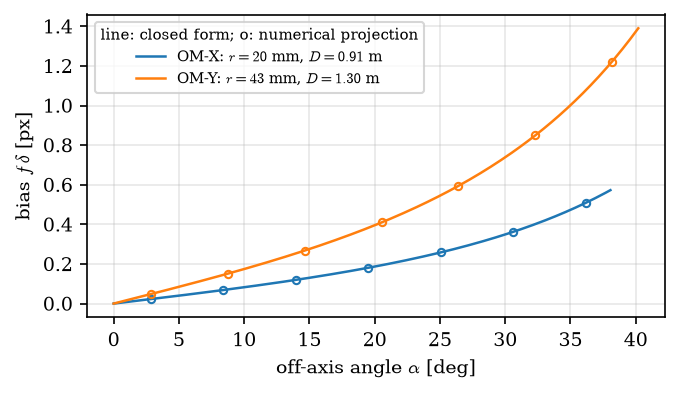
\includegraphics[width=0.62\linewidth]{figures/perspective_bias.png}
\caption{Perspective bias $f\delta$ (Eq.~\ref{eq:bias}) between the
silhouette centre and the projection of the sphere centre, at the default-pose
distance. Circles are the independent numerical check.}
\label{fig:bias}
\end{figure}

\begin{proposition}[MEC under occlusion]
\label{prop:occlusion}
Let $\mathcal D$ be the silhouette disk (radius $R$, centre $\vect c$) and
$S\subseteq\mathcal D$ the compact visible part.
\begin{enumerate}
\item[(i)] If $S$ contains two antipodal points of $\partial\mathcal D$ (for
example, a border arc of angle $\geq\pi$), then $\MEC(S)=\mathcal D$ and the
estimated centre is exact.
\item[(ii)] If the occluder is a half-plane and less than half the disk is
visible, $S=\mathcal D\cap\{\vect x:\langle\vect x-\vect c,\vect n\rangle\leq-h\}$
with $0<h<R$ and $\|\vect n\|=1$, then $\MEC(S)$ is the disk with the chord as
diameter: centre $\vect c-h\vect n$, radius $\sqrt{R^2-h^2}$. The centre error
is $h$, and the visible fraction is
$f(h)=\bigl[\arccos(h/R)-(h/R)\sqrt{1-h^2/R^2}\bigr]/\pi$.
\end{enumerate}
\end{proposition}
\begin{proof}
(i) Any disk containing two points at distance $2R$ has radius $\geq R$, and
$\mathcal D\supseteq S$ has radius $R$. By uniqueness, $\MEC(S)=\mathcal D$.
(ii) Write $\vect x\in S$ as $\vect x=\vect c-s\vect n+w\vect\tau$ with
$\vect\tau\perp\vect n$, $s\geq h$, and $s^2+w^2\leq R^2$. Then
$\|\vect x-(\vect c-h\vect n)\|^2=(s-h)^2+w^2\leq(s-h)^2+R^2-s^2=R^2-h^2-2h(s-h)\leq
R^2-h^2$, so the proposed disk contains $S$. The chord endpoints, $s=h$ and
$w=\pm\sqrt{R^2-h^2}$, are antipodal on it, and the argument of (i) concludes.
\end{proof}

Proposition~\ref{prop:occlusion} shows the advantage of the MEC over the
centroid (first-order moments). With up to half the disk hidden by a straight
edge, the MEC stays exact, while the centroid of a half disk is already off
by $4R/(3\pi)\approx0.42R$. Figure~\ref{fig:circ}(b) compares both for a digital
disk with $R=30$\,px. In regime (i) the measured MEC error stays
$\leq\num{\CircMecErrAboveHalfMax}R$. The residual gap to the theory comes from
conditioning: near the widest chord, the distance to the extreme points
changes only to second order with the centre position, so a digitisation
perturbation $\varepsilon$ moves the centre by about $\sqrt{2R\varepsilon}$
(heuristic estimate; for $\varepsilon\approx0.07$\,px, $\approx2$\,px).
Circularity decreases monotonically with occlusion (dash-dot curve), which
partly justifies using it as a confidence.

\begin{figure}[ht]
\centering
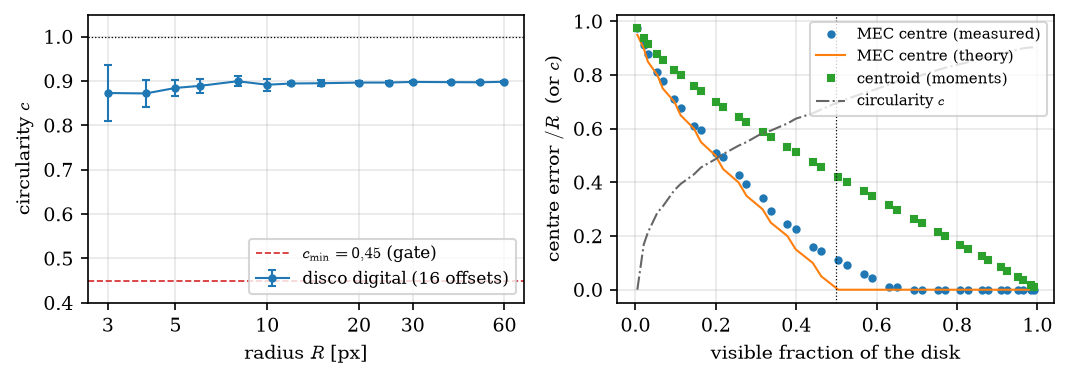
\includegraphics[width=\linewidth]{figures/circularity.png}
\caption{(a) Circularity of digital disks against radius (mean and standard
deviation over 16 sub-pixel offsets); the asymptote is $c_\infty\approx0.899$
(Proposition~\ref{prop:circ-digital}). (b) Half-plane occlusion of a disk with
$R=30$\,px: MEC centre error (measured and theoretical,
Proposition~\ref{prop:occlusion}), centroid error, and circularity.}
\label{fig:circ}
\end{figure}

%=====================================================================
\section{From pixel to world: lifting to the table plane}
\label{sec:lift}
%=====================================================================

\subsection{Back-projection}

The pixel $(\hat u,\hat v)$ defines the ray
\begin{equation}
\vect x(\lambda)=\vect O+\lambda\,\vect d,\qquad
\vect d=R\,K^{-1}\tilde{\vect u}=R\begin{bmatrix}(\hat u-c_x)/f_x\\(\hat v-c_y)/f_y\\1\end{bmatrix},\qquad\lambda>0.
\label{eq:ray}
\end{equation}
The code normalises $\vect d$ (\code{_pixel_ray_cam}). That changes the
parameter $\lambda$ but not the intersection point. With the unnormalised form
of \eqref{eq:ray}, since the third component of $K^{-1}\tilde{\vect u}$ is 1,
the value of $\lambda$ at the intersection equals the depth $Z$ of the point
in $\{C\}$.

\subsection{The plane of centres}

A sphere of radius $r$ resting on a horizontal plane at height
$z_{\text{table}}$ has its centre at $z=z_{\text{table}}+r$. The lifter uses the
plane
\begin{equation}
\Pi=\{\vect x\in\R^3:\ \ez\T\vect x=z_\Pi\},\qquad z_\Pi=z_{\text{table}}+r,
\end{equation}
with $z_{\text{table}}=0$ and $r=\SI{\OmxBallr}{mm}$ (OM-X) or
\SI{\OmyBallr}{mm} (OMY), read from \code{lifter} in the YAML. The
intersection is
\begin{equation}
\lambda^\star=\frac{z_\Pi-O_z}{d_z},\qquad \hat{\vect p}=\vect O+\lambda^\star\vect d,
\label{eq:lift}
\end{equation}
defined when $|d_z|\geq10^{-12}$ (ray not parallel to the plane) and
$\lambda^\star>0$ (plane in front of the camera). Otherwise the view is
discarded (\code{intersect_ray_horizontal_plane}).

\begin{proposition}[Model exactness]
\label{prop:exact}
If the true centre $\vect p^\star$ lies on $\Pi$, is in front of the camera,
and $(\hat u,\hat v)=\pi(\vect p^\star)$ is its exact projection by
Eq.~\eqref{eq:proj}, then Eq.~\eqref{eq:lift} returns $\hat{\vect p}=\vect p^\star$.
\end{proposition}
\begin{proof}
By definition of central projection, $\vect p^\star=\vect O+Z^\star\vect d$
with $\vect d$ from \eqref{eq:ray} and $Z^\star>0$. Since $d_z\neq0$, the line
meets $\Pi$ in exactly one point, which is therefore $\vect p^\star$.
\end{proof}

So, with a single camera, position error comes from only three sources:
centre pixel error (bias from Proposition~\ref{prop:ellipse}, occlusion,
digitisation), plane-model error ($z_\Pi$), and calibration error. Each is
quantified in Section~\ref{sec:error}. An important consequence is that the
estimated height is always $z_\Pi$ by construction, so the $z$ error is zero
as long as the ball really rests on the table.

\subsection{Multi-view fusion}
\label{sec:fusion}

For each configured camera $i$ that produced a detection, the lifter keeps
the one with highest confidence (the detector already returns at most one),
computes $\hat{\vect p}_i$ by \eqref{eq:lift}, and fuses
\begin{equation}
\hat{\vect p}=\sum_i w_i\,\hat{\vect p}_i,\qquad
w_i=\frac{\max(\kappa_i,10^{-3})}{\sum_j\max(\kappa_j,10^{-3})},
\label{eq:fuse}
\end{equation}
then re-imposes $\hat p_z=z_\Pi$ (\code{TablePlanePoseLifter.lift}). Since
$\Pi$ is affine and \eqref{eq:fuse} is a convex combination of points of
$\Pi$, the re-imposition only removes rounding. One view is enough: if one
camera is obstructed, the other alone defines $\hat{\vect p}$.

\begin{remark}[Optimal weights]
If the $\hat{\vect p}_i$ were unbiased and independent with in-plane
covariances $\Sigma_i$, the minimum-variance linear estimator would be
$\hat{\vect p}=(\sum_i\Sigma_i^{-1})^{-1}\sum_i\Sigma_i^{-1}\hat{\vect p}_i$.
Eq.~\eqref{eq:fuse} uses scalar weights based on circularity rather than on
$\Sigma_i$. The two coincide when the views have equal covariances. Without
occlusion, $\kappa_L\approx\kappa_R\approx0.89$ and the weights are
$\approx\frac12$.
\end{remark}

The output is a \code{BallObservation} with \code{position_world}$=\hat{\vect
p}$, \code{radius_m}$=r$, \code{timestamp} equal to the latest timestamp among
the frames used, and \code{source} equal to the pipeline id. The
\code{covariance} field exists in the type but the current lifter does not
fill it (Section~\ref{sec:error} shows how to compute it), and \code{pickable}
stays \code{None}.

\subsection{Complete numerical example}
\label{sec:example}

Table~\ref{tab:example} follows the computation in the OM-X cell with the ball
at the default pick pose,
$\vect p^\star=(\num{\OmxGtX}, \num{\OmxGtY}, \num{\OmxGtZ})$\,mm. Every value
comes from the real pipeline; the step-by-step re-implementation used to fill
the table reproduces the detector mask bit for bit and the fused position to
$10^{-12}$\,m.

\begin{table}[ht]
\centering
\small
\caption{Complete example, OM-X, pose \code{pick_default}. Lengths in metres
unless stated.}
\label{tab:example}
\begin{tabular}{@{}lcc@{}}
\toprule
& left camera ($L$) & right camera ($R$)\\
\midrule
contours found & \num{\OmxLNContours} & \num{\OmxRNContours}\\
area $A$ / perimeter $P$ [px] & \num{\OmxLAreaPx} / \num{\OmxLPerimeterPx} & \num{\OmxRAreaPx} / \num{\OmxRPerimeterPx}\\
circularity $c=\kappa$ & \num{\OmxLCirc} & \num{\OmxRCirc}\\
IoU mask vs.\ segmentation & \num{\OmxLIou} & \num{\OmxRIou}\\
MEC centre $(\hat u,\hat v)$ [px] & (\num{\OmxLU}, \num{\OmxLV}) & (\num{\OmxRU}, \num{\OmxRV})\\
exact projection $\pi(\vect p^\star)$ [px] & (\num{\OmxLUGt}, \num{\OmxLVGt}) & (\num{\OmxRUGt}, \num{\OmxRVGt})\\
centre error [px] & \num{\OmxLCentreErrPx} & \num{\OmxRCentreErrPx}\\
predicted bias $f\delta$ (Eq.~\ref{eq:bias}) [px] & \num{\OmxLEllBias} & \num{\OmxREllBias}\\
MEC radius $\hat\rho$ / predicted $fa$ [px] & \num{\OmxLRadiusPx} / \num{\OmxLEllA} & \num{\OmxRRadiusPx} / \num{\OmxREllA}\\
\midrule
$K^{-1}\tilde{\vect u}$ & (\num{\OmxLDcX}, \num{\OmxLDcY}, \num{\OmxLDcZ}) & (\num{\OmxRDcX}, \num{\OmxRDcY}, \num{\OmxRDcZ})\\
$\vect d=RK^{-1}\tilde{\vect u}$ & (\num{\OmxLDwX}, \num{\OmxLDwY}, \num{\OmxLDwZ}) & (\num{\OmxRDwX}, \num{\OmxRDwY}, \num{\OmxRDwZ})\\
optical centre $\vect O$ & (\num{\OmxLOX}, \num{\OmxLOY}, \num{\OmxLOZ}) & (\num{\OmxROX}, \num{\OmxROY}, \num{\OmxROZ})\\
$\lambda^\star=(z_\Pi-O_z)/d_z$ & \num{\OmxLT} & \num{\OmxRT}\\
depth $Z$ of $\vect p^\star$ & \num{\OmxLDepth} & \num{\OmxRDepth}\\
$\hat{\vect p}_i$ [mm] & (\num{\OmxLPX}, \num{\OmxLPY}, \num{\OmxLPZ}) & (\num{\OmxRPX}, \num{\OmxRPY}, \num{\OmxRPZ})\\
weight $w_i$ & \num{\OmxLWeight} & \num{\OmxRWeight}\\
\midrule
fused $\hat{\vect p}$ [mm] & \multicolumn{2}{c}{(\num{\OmxFuX}, \num{\OmxFuY}, \num{\OmxFuZ})}\\
error $\|\hat{\vect p}-\vect p^\star\|_{xy}$ / $|\Delta z|$ [mm] & \multicolumn{2}{c}{\num{\OmxExXyerr} / \num{\OmxExZerr}}\\
\bottomrule
\end{tabular}
\end{table}

Note that $\lambda^\star$ equals the depth $Z$, as predicted. In the OMY cell,
at the default pose $(\num{\OmyGtX}, \num{\OmyGtY})$\,mm, the same computation
gives $\hat{\vect p}=(\num{\OmyFuX}, \num{\OmyFuY}, \num{\OmyFuZ})$\,mm, a
horizontal error of \SI{\OmyExXyerr}{mm}. Figure~\ref{fig:geom} shows the rays
and the in-plane errors.

\begin{figure}[ht]
\centering
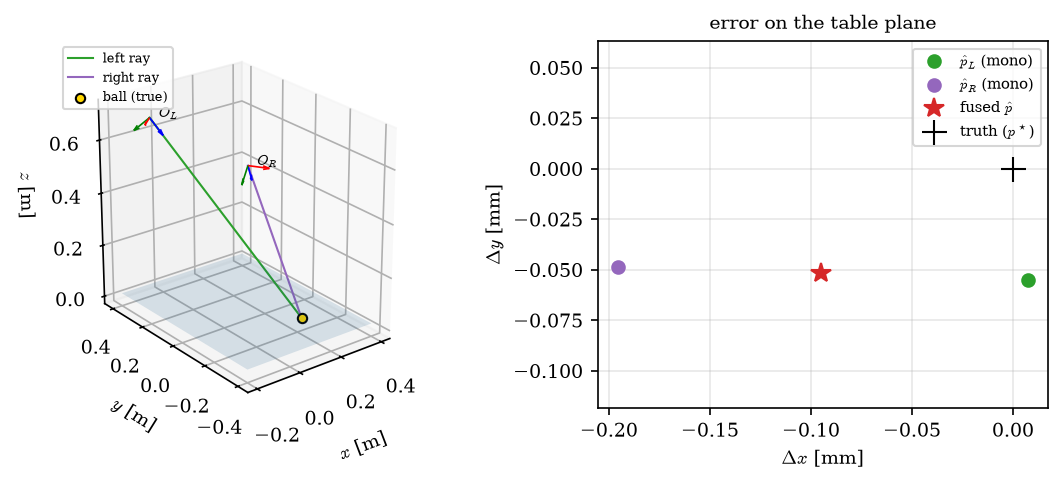
\includegraphics[width=\linewidth]{figures/geometry_omx.png}
\caption{Left: back-projection rays of both cameras (axes $x_C,y_C,z_C$ in
red, green, blue) down to the plane $\Pi$ (OM-X). Right: error of the
monocular and fused estimates on the table plane, in millimetres.}
\label{fig:geom}
\end{figure}

%=====================================================================
\section{Error analysis}
\label{sec:error}
%=====================================================================

\subsection{Jacobian of the lift}

\begin{proposition}
\label{prop:jac}
Let $\vect r_k$ be the $k$-th column of $R$. The derivative of the point
\eqref{eq:lift} with respect to the pixel is
\begin{equation}
\frac{\partial\hat{\vect p}}{\partial u}=\frac{\lambda^\star}{f_x}\Bigl(\vect r_1-\frac{r_{1z}}{d_z}\vect d\Bigr),\qquad
\frac{\partial\hat{\vect p}}{\partial v}=\frac{\lambda^\star}{f_y}\Bigl(\vect r_2-\frac{r_{2z}}{d_z}\vect d\Bigr),
\label{eq:jac}
\end{equation}
with zero $z$ component. Define $J=[\partial_u\hat{\vect p}\ \ \partial_v\hat{\vect p}]_{xy}\in\R^{2\times2}$.
\end{proposition}
\begin{proof}
From \eqref{eq:ray}, $\partial\vect d/\partial u=\vect r_1/f_x$. From
\eqref{eq:lift}, $\partial\lambda^\star/\partial u=-\lambda^\star(\partial
d_z/\partial u)/d_z=-\lambda^\star r_{1z}/(f_xd_z)$. By the product rule,
$\partial\hat{\vect p}/\partial u=(\partial\lambda^\star/\partial u)\vect d+
\lambda^\star\partial\vect d/\partial u$, which is the first expression. Its
$z$ component is $\frac{\lambda^\star}{f_x}(r_{1z}-r_{1z})=0$. The $v$ case is
analogous.
\end{proof}

In the example, in mm/px,
\[
J_L=\begin{bmatrix}\num{\OmxLJAa}&\num{\OmxLJAb}\\ \num{\OmxLJBa}&\num{\OmxLJBb}\end{bmatrix},\qquad
J_R=\begin{bmatrix}\num{\OmxRJAa}&\num{\OmxRJAb}\\ \num{\OmxRJBa}&\num{\OmxRJBb}\end{bmatrix},
\]
with largest singular values \num{\OmxLJsig} and \num{\OmxRJsig}\,mm/px.
Formula \eqref{eq:jac} agrees with central finite differences to
\num{\OmxJacFd}\,m/px. Figure~\ref{fig:sens} maps $\sigma_{\max}(J)$ over the
table. Sensitivity grows with distance and with ray obliquity, and fusion with
equal weights reduces the covariance.

\begin{figure}[ht]
\centering
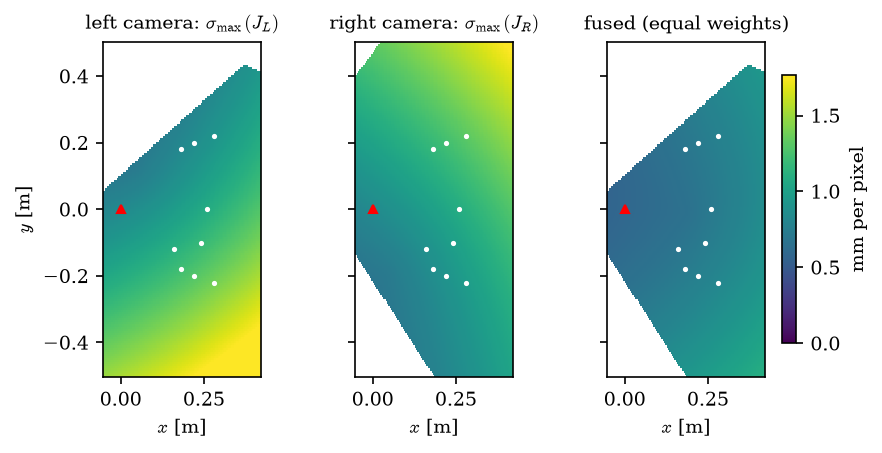
\includegraphics[width=\linewidth]{figures/sensitivity_omx.png}\\[2pt]
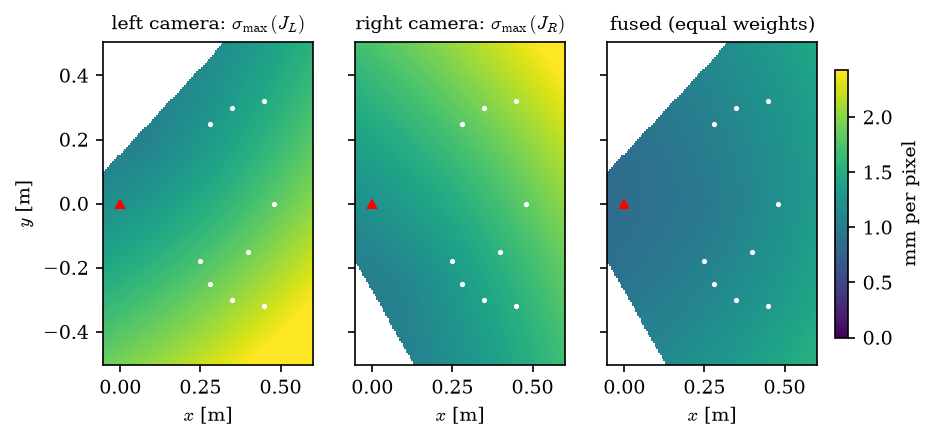
\includegraphics[width=\linewidth]{figures/sensitivity_omy.png}
\caption{Sensitivity $\sigma_{\max}(J)$ of the lifted point to pixel error
(mm/px) over the plane $\Pi$, only where the point projects inside the image.
Top: OM-X; bottom: OMY. White dots: sweep poses of
Section~\ref{sec:results}; triangle: arm base. The map ignores occlusion by
the robot.}
\label{fig:sens}
\end{figure}

\subsection{Covariance propagation and Monte Carlo check}

If the centre error in each view is independent with covariance
$\sigma^2I_2$, linearisation gives
\begin{equation}
\Sigma_i\approx\sigma^2J_iJ_i\T,\qquad \Sigma_{\hat{\vect p}}\approx\sum_iw_i^2\,\Sigma_i.
\label{eq:cov}
\end{equation}
To check \eqref{eq:cov}, we add Gaussian noise with $\sigma=0.5$\,px to the
detected centres of the example, repeat lift and fusion \num{20000} times, and
compare the empirical covariance with the prediction. The semi-axes of the
$1\sigma$ ellipse were (\num{\OmxMcEmpMinMm}, \num{\OmxMcEmpMaxMm})\,mm
(empirical) and (\num{\OmxMcPredMinMm}, \num{\OmxMcPredMaxMm})\,mm (predicted),
with a relative Frobenius difference of \num{\OmxMcFrobRel} (OMY:
(\num{\OmyMcEmpMinMm}, \num{\OmyMcEmpMaxMm}) vs.\ (\num{\OmyMcPredMinMm},
\num{\OmyMcPredMaxMm})\,mm). Linearisation is therefore excellent at this
scale, and \eqref{eq:cov} could fill the \code{covariance} field of
\code{BallObservation}.

\subsection{Plane-model error}

If the true centre is at $z_\Pi+\delta z$ (wrong configured radius, higher
table, or ball on a support), the ray through the true centre meets $\Pi$ at
$\vect p^\star-(\delta z/d_z)\vect d$. The horizontal error is
\begin{equation}
\Delta\hat{\vect p}_{xy}=-\delta z\,\frac{\vect d_{xy}}{d_z},\qquad
\|\Delta\hat{\vect p}_{xy}\|=|\delta z|\tan\theta,
\end{equation}
with $\theta$ the angle of the ray from the vertical. In the example,
$\tan\theta_L=\num{\OmxLTanIncidence}$ and $\tan\theta_R=\num{\OmxRTanIncidence}$.
In the fusion the shifts are vectors and partly cancel because the cameras are
on opposite sides: the fused error is \num{\OmxDzShift}\,mm per millimetre of
$\delta z$ (OMY: \num{\OmyDzShift}). For example, a \SI{1}{mm} error in the
configured ball radius shifts the estimate by $\approx\SI{0.6}{mm}$.

\subsection{Calibration error}

A small camera rotation $\delta\phi$ deflects every ray by the same angle,
which to first order equals a pixel shift of $f\,\delta\phi$. With
$f\approx938$\,px and $\sigma_{\max}(J)\approx1.3$\,mm/px, \SI{1}{mrad} of
orientation error is worth $\approx\SI{0.94}{px}\approx\SI{1.2}{mm}$. A
translation error $\delta\vect O$ moves $\hat{\vect p}$ by
$\delta\vect O_{xy}-\delta O_z\,\vect d_{xy}/d_z$. In simulation both are zero
to \num{e-10} (Section~\ref{sec:camera}). In a real cell, extrinsic
calibration is likely to be the dominant error source.

\subsection{Partial occlusion: case study}
\label{sec:occlusion-case}

The worst case of the sweep is the OM-X \code{mid_backish} pose, with the
ball at $(0.16, -0.12)$\,m (Figure~\ref{fig:occlusion}). On the left camera the
arm hides most of the ball: only \SI{\OccVisibleFrac}{\percent} of the
theoretical silhouette is visible. The circularity of the visible part is
\num{\OccCirc}, above $c_{\min}=0.45$, so the detection is accepted. The MEC
falls in regime (ii) of Proposition~\ref{prop:occlusion}. With a straight
occluder the model would predict $h\approx14$\,px for that visible fraction;
the measured centre error is \num{\OccCentreErrPx}\,px (the arm edge is not
straight). The left monocular estimate is off by \SI{\occLeftErr}{mm}, while
the unoccluded right one is off by \SI{\occMonoErr}{mm}. Because the low
circularity gives weight $w_L=\num{\occLeftW}$, fusion attenuates but does not
remove the error: the fused result is off by \SI{\occFusedErr}{mm}. That is
still within the \SI{15}{mm} benchmark tolerance, but it exposes the weak spot
of the weighting scheme (Section~\ref{sec:limitations}).

\begin{figure}[ht]
\centering
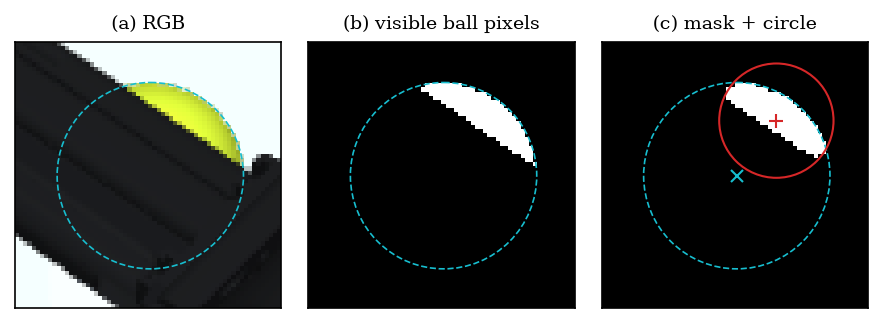
\includegraphics[width=0.78\linewidth]{figures/occlusion_omx.png}
\caption{Partial occlusion by the arm (OM-X, \code{mid_backish}, left
camera). Dashed cyan: full theoretical silhouette
(Proposition~\ref{prop:ellipse}); $\times$: exact projection of the centre;
red: MEC of the mask and estimated centre.}
\label{fig:occlusion}
\end{figure}

%=====================================================================
\section{Results in simulation}
\label{sec:results}
%=====================================================================

Tables~\ref{tab:sweep-omx} and~\ref{tab:sweep-omy} repeat the nine poses of
\code{scripts/benchmark_mujoco_vision.py}. For each camera, the ``visible''
column is the ratio between the ball pixels in the reference segmentation and
the theoretical silhouette area $\pi f^2ab$. It measures occlusion directly.

\begin{table}[ht]
\centering
\footnotesize
\caption{OM-X sweep ($L$ / $R$ = left / right camera). XY error of the fused
estimate against the true MuJoCo ball position.}
\label{tab:sweep-omx}
\begin{tabular}{@{}lcccccc@{}}
\toprule
pose & $(x,y)$ [m] & views & visible [\%] & $c$ & centre error [px] & XY error [mm]\\
\midrule
\generatedrows{sweep_omx.tex}
\bottomrule
\end{tabular}
\end{table}

\begin{table}[ht]
\centering
\footnotesize
\caption{OMY sweep. In \code{front_cone} the ball is inside the place bin
(\SI{0.28}{m} walls); only a cap of about \SI{11}{\percent} shows above the
wall, and it does not pass the area and circularity filters. The pipeline
returns \code{None} and does not invent a pose.}
\label{tab:sweep-omy}
\begin{tabular}{@{}lcccccc@{}}
\toprule
pose & $(x,y)$ [m] & views & visible [\%] & $c$ & centre error [px] & XY error [mm]\\
\midrule
\generatedrows{sweep_omy.tex}
\bottomrule
\end{tabular}
\end{table}

For a spatial view, Figure~\ref{fig:maps} sweeps the ball over a dense grid:
\num{\OmxGridN} positions for OM-X and \num{\OmyGridN} for OMY, with the arm in
its sensing configuration. When both cameras see more than
\SI{95}{\percent} of the silhouette (\num{\OmxGridClearN} positions for OM-X and
\num{\OmyGridClearN} for OMY), the XY error has median
\SI{\OmxGridClearMedian}{mm} and maximum \SI{\OmxGridClearMax}{mm} (OM-X), and
median \SI{\OmyGridClearMedian}{mm} and maximum \SI{\OmyGridClearMax}{mm} (OMY),
consistent with the pixel analysis of Section~\ref{sec:error}. Elsewhere the
errors cluster in well-defined bands where the arm or the bin walls cover part
of the ball in one view (regime (ii) of Proposition~\ref{prop:occlusion}). Over
the full grid, the median is \SI{\OmxGridMedian}{mm} and the 95th percentile
\SI{\OmxGridPjf}{mm} (OM-X); for OMY, the median is \SI{\OmyGridMedian}{mm} and
the 95th percentile \SI{\OmyGridPjf}{mm}. OM-X detects the ball at all
\num{\OmxGridN} positions, and OMY at \num{\OmyGridDet} of \num{\OmyGridN}. The
OMY misses are inside the place bin or in the corner $x\approx0.15$\,m,
$y\approx0.4$\,m, where no camera has an unobstructed view.

\begin{figure}[ht]
\centering
\begin{subfigure}{0.49\linewidth}
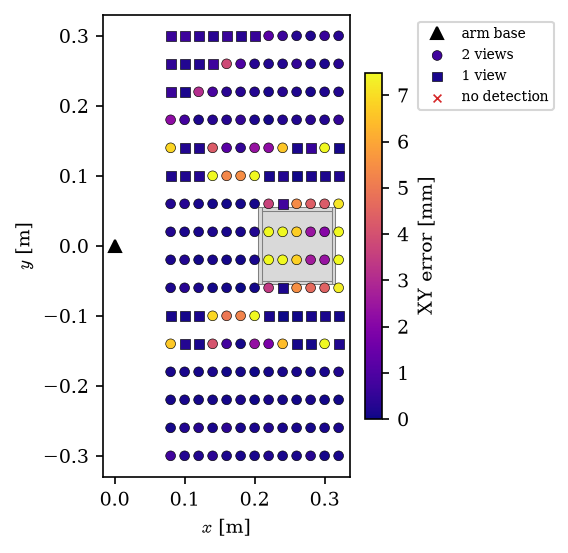
\includegraphics[width=\linewidth]{figures/error_map_omx.png}
\caption{OM-X}
\end{subfigure}\hfill
\begin{subfigure}{0.49\linewidth}
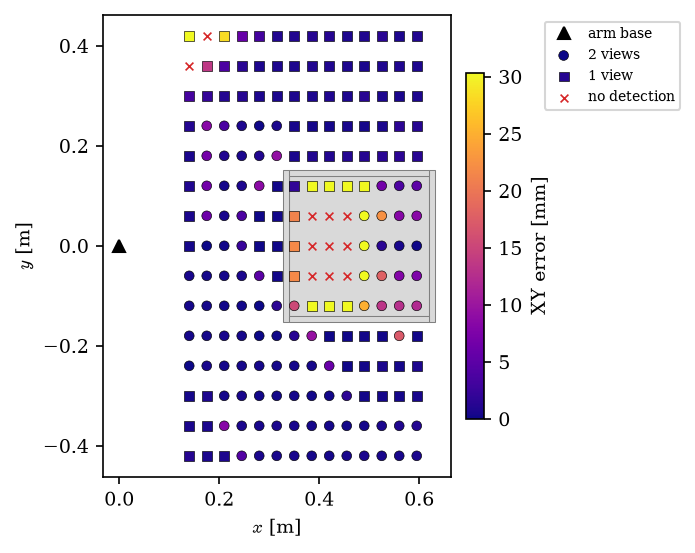
\includegraphics[width=\linewidth]{figures/error_map_omy.png}
\caption{OMY}
\end{subfigure}
\caption{XY error of the fused estimate over a dense grid of ball positions.
Circle: two views; square: one view; $\times$: no detection. Grey: place bin.
The colour scale saturates at the 95th percentile.}
\label{fig:maps}
\end{figure}

%=====================================================================
\section{From ball position to grasp pose}
\label{sec:grasp}
%=====================================================================

\subsection{Why position is enough}

A homogeneous sphere is invariant under any rotation about its own centre.
The action of $SE(3)$ on the sphere has stabiliser $SO(3)$ (rotations about
the centre), and the space of distinguishable poses is the quotient
$SE(3)/SO(3)\cong\R^3$. The object ``pose'' is therefore exactly the centre
position $\hat{\vect p}$, which is what \code{BallObservation} carries. Vision
does not impose the gripper orientation: it is free and chosen by inverse
kinematics.

\subsection{Cartesian targets}

From $\hat{\vect p}$, \code{_pad_mid_pick_waypoints}
(\code{fret/control/pick_place_vision.py}) defines three targets for the
midpoint between the fingertips:
\begin{equation}
\vect p_{\text{hover}}=\hat{\vect p}+h_{\text{hover}}\ez,\qquad
\vect p_{\text{grasp}}=\hat{\vect p}+0.012\,\ez,\qquad
\vect p_{\text{lift}}=\hat{\vect p}+h_{\text{lift}}\ez,
\end{equation}
with $(h_{\text{hover}},h_{\text{lift}})=(0.08, 0.12)$\,m for OM-X and
$(0.10, 0.14)$\,m for OMY. The \SI{12}{mm} offset above the centre at grasp
lets the fingers close on the sphere without touching the table. The gripper
opening is fixed per target: open at hover, closed (``pinch'') at grasp and
lift.

\subsection{Fingertip-midpoint inverse kinematics}

Let $\vect m(\vect q)=\frac12\bigl(\vect x_{\text{R}}(\vect q)+\vect x_{\text{L}}(\vect q)\bigr)$
be the midpoint of the \code{pad_right} and \code{pad_left} geom centres,
computed by MuJoCo forward kinematics, with $\vect q\in\R^n$ ($n=4$ for OM-X,
$n=6$ for OMY). For each target $\vect p_\ast$ we solve
\begin{equation}
\vect q_\ast=\argmin_{\vect q\in[\vect q_{\min},\vect q_{\max}]}\ \|\vect m(\vect q)-\vect p_\ast\|^2
\label{eq:ik}
\end{equation}
with L-BFGS-B \cite{byrd1995} (\code{pad_mid_ik},
\code{fret/control/omy_pad_mid_ik.py}) from several seeds: the previous
target's solution (warm start), the scenario YAML configurations, and
robot-specific seeds. The lowest-residual solution is kept. If the residual
$\|\vect m(\vect q_\ast)-\vect p_\ast\|$ exceeds \SI{8}{mm}, the routine raises
instead of sending a poor grasp. Because OM-X has 4 degrees of freedom and the
target has 3 dimensions, \eqref{eq:ik} generally has a family of solutions;
the seeds select among them. In the example of Table~\ref{tab:example}, the
residuals were \SI{\OmxIkHoverMm}{mm} (hover), \SI{\OmxIkGraspMm}{mm} (grasp),
and \SI{\OmxIkLiftMm}{mm} (lift) for OM-X, and $\leq\SI{\OmyIkGraspMm}{mm}$ for
OMY. Cartesian positioning error is therefore dominated by vision, not by IK.

\subsection{Integration with the state machine}

In the simulators (\code{simulate_pick_place} and
\code{simulate_omy_pick_place}), vision runs once, before the arm folds into
its idle posture. The order matters because the folded posture occludes one
camera. \code{apply_vision_pick_goals} renders the cameras, runs the pipeline,
and raises if there is no \code{BallObservation}: the system never grasps
blind. With an observation, it replaces the state machine's pick
configurations (the place configurations still come from the YAML, because the
place bin is a known fixture) and moves the visual \code{cv_ball_ghost} sphere
to $\hat{\vect p}$ (Figure~\ref{fig:overview}).

%=====================================================================
\section{Limitations and possible improvements}
\label{sec:limitations}
%=====================================================================

\begin{enumerate}
\item \textbf{Cross-view association.} Each camera picks its own blob with
the highest circularity, and nothing checks that the views saw the same
object. With two balls visible, Eq.~\eqref{eq:fuse} can average two different
objects and produce a point between them. A consistency test
$\|\hat{\vect p}_L-\hat{\vect p}_R\|\leq\tau$ (for example
$\tau=3\sqrt{\operatorname{tr}(\Sigma_L+\Sigma_R)}$) would catch this case.
\item \textbf{Partial occlusion.} Circularity only reduces the weight of an
occluded view (Section~\ref{sec:occlusion-case}). Alternatives: reject views
whose $\hat\rho$ is much smaller than the predicted radius $f\,a(\hat{\vect p})$
(Corollary~\ref{cor:mec-ellipse} gives the prediction from the other view's
estimate), use minimum-variance weights with $\Sigma_i$ inflated by $1/c_i$,
or apply the consistency test of the previous item.
\item \textbf{Perspective bias.} At most $\approx\SI{1.4}{px}$; it can be
corrected in closed form with Eq.~\eqref{eq:bias}.
\item \textbf{Plane assumption.} The $z$ estimate is imposed. A ball off the
table (on an obstacle, or in the air) causes a horizontal error of
$\delta z\tan\theta$. With two views, least-squares triangulation could
estimate $z$ and serve as a diagnostic.
\item \textbf{Colour and lighting.} The HSV threshold is fixed. It works well
in simulation (Figure~\ref{fig:hsv}), but real cameras need colour
calibration and a lens-distortion model, which is absent today.
\item \textbf{Uncertainty.} The \code{covariance} field can be filled with
Eq.~\eqref{eq:cov}, validated by the Monte Carlo experiment.
\end{enumerate}

%=====================================================================
\appendix
\section{Configuration parameters}
\label{app:params}
%=====================================================================

\begin{table}[H]
\centering
\small
\begin{tabular}{@{}lll@{}}
\toprule
parameter & OM-X (\code{omx_portal_overhead.yml}) & OMY (\code{omy_portal_overhead.yml})\\
\midrule
resolution & $1280\times720$ & $1280\times720$\\
\code{fovy} / $f$ [px] & \ang{\OmxFovy} / \num{\OmxFx} & \ang{\OmyFovy} / \num{\OmyFx}\\
optical centres $\vect O$ [m] & $(-0.12,\ \pm0.30,\ 0.70)$ & $(-0.18,\ \pm0.42,\ 0.98)$\\
$\vect\ell$ / $\vect h$ (HSV) & $(20,40,40)$ / $(50,255,255)$ & $(20,40,40)$ / $(50,255,255)$\\
structuring element & elliptical $5\times5$ & elliptical $5\times5$\\
$A_{\min}$ / $A_{\max}$ [px$^2$] & 80 / \num{500000} & 120 / \num{500000}\\
$c_{\min}$ & 0.45 & 0.45\\
$z_{\text{table}}$ / $r$ [m] & 0 / 0.020 & 0 / 0.043\\
\bottomrule
\end{tabular}
\caption{Pipeline parameters for the two gate cells. \code{config/vision/}
also has \code{hsv_blob_overhead.yml} (synthetic fixture, $640\times480$,
$c_{\min}=0.55$) and \code{hsv_blob_tennis_yellow.yml} (web photos).}
\end{table}

\section{Reproducibility}

Every figure, table, and number in this document is generated by
\begin{verbatim}
MUJOCO_GL=egl PYOPENGL_PLATFORM=egl python3 scripts/vision_algorithm_figures.py
cd docs/vision/algorithm && latexmk -pdf vision_algorithm.tex
\end{verbatim}
The script uses the production pipeline (\code{pipeline_from_hsv_plane_config})
and asserts that the step-by-step re-implementation matches it: identical
mask, same detection centre, and fused position equal to $10^{-12}$\,m. Raw
metrics are in \code{metrics.json}. The same run renders
\code{vision_algorithm.md} from \code{vision_algorithm.template.md}.

\begin{thebibliography}{9}
\bibitem{hartley2004} R.~Hartley and A.~Zisserman. \emph{Multiple View Geometry
in Computer Vision}, 2nd ed. Cambridge University Press, 2004.
\bibitem{serra1982} J.~Serra. \emph{Image Analysis and Mathematical Morphology}.
Academic Press, 1982.
\bibitem{suzuki1985} S.~Suzuki and K.~Abe. Topological structural analysis of
digitized binary images by border following. \emph{Computer Vision, Graphics,
and Image Processing}, 30(1):32--46, 1985.
\bibitem{welzl1991} E.~Welzl. Smallest enclosing disks (balls and ellipsoids).
In \emph{New Results and New Trends in Computer Science}, LNCS 555, pp.~359--370.
Springer, 1991.
\bibitem{smith1978} A.~R.~Smith. Color gamut transform pairs. \emph{ACM SIGGRAPH
Computer Graphics}, 12(3):12--19, 1978.
\bibitem{freeman1961} H.~Freeman. On the encoding of arbitrary geometric
configurations. \emph{IRE Trans. Electronic Computers}, EC-10(2):260--268, 1961.
\bibitem{byrd1995} R.~H.~Byrd, P.~Lu, J.~Nocedal, and C.~Zhu. A limited memory
algorithm for bound constrained optimization. \emph{SIAM J. Sci. Comput.},
16(5):1190--1208, 1995.
\bibitem{opencv} G.~Bradski. The OpenCV Library. \emph{Dr.\ Dobb's Journal of
Software Tools}, 2000.
\end{thebibliography}

\end{document}
